\begin{problem}
Use a discrete version of the one-point exchange algorithm to calculate the best minimax approximation from the space of polynomials of degree at most one to the following seven function values: $f(0)=0.3, f(1) = 4.2, f(2) = 0.1, f(3) = 3.4, f(4) = 5.7, f(5) = 4.9, f(6) = 5.7$. Let the initial reference be the set of points $\{0, 3, 6\}$.
\end{problem}

\begin{solution}
When we are given a set of functional values on a grid:
\begin{equation*}
\mathcal{G} = \{x_1,x_2,\ldots,x_m\} \subset [a,b] \quad m>dim(\mathcal{A})
\end{equation*}
we modify the method with $\mathcal{Z} \subset \mathcal{G}$. Let us consider the monomial basis $\{1,x\}$ and solve the equation system:
\begin{equation*}
f(\xi_i)=\lambda_0+\lambda_1\xi_i + (-1)^ih
\end{equation*}
On the first iteration we obtain the solution $p(x) = 0.5 + 0.9x$ with $h=-0.2$ and change the reference to $\{0, 1, 6\}$ (the closest point $\xi$ of the error function with the same sign as $\eta$). On the fourth iteration we finally arrive at the best minimax approximation (the discrete algorithm always finds the best minimax approximation in a finite number of steps), that is $p(x) = 1.4 + 0.5x$ with $h = 2.3$ on the reference $\{1, 2, 4\}$ as we can see in Figure \ref{discreteminimax}.
\begin{figure}[h]
\centering 
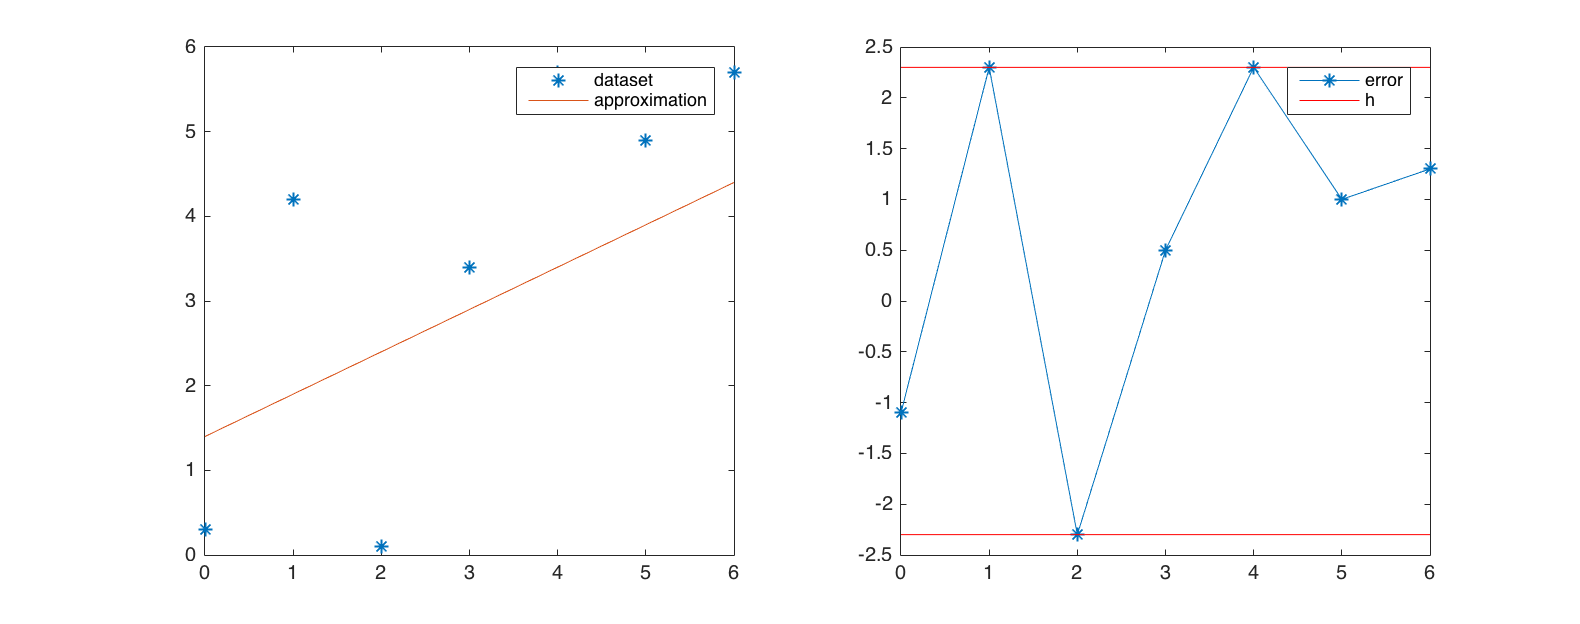
\includegraphics[scale = 0.25]{hwk5t3.png}
\caption{plot of the dataset approximated by $1.4 + 0.5x$, error and $h$. Reference $\{1,2,4\}$}
\label{discreteminimax}
\end{figure}
\end{solution}

%%% Local Variables:
%%% mode: latex
%%% TeX-master: "report"
%%% End:
